\subsection*{Assignment 21 -- Grafici delle Stream Totali e Numero di Canzoni Explicit}
L'Assignment 21 richiedeva di creare un grafico o una dashboard
che fornisca informazioni sui dati testuali presenti nel datacube.
A questo scopo, è stato ritenuto interessante proporre dei grafici
che rappresentano la distribuzione degli ascolti e del numero di
canzoni explicit, rispetto a quelle che invece non lo sono.
La Figura~\ref{fig:ass_21} riporta i grafici che descrivono questi dati.

\begin{figure}[H]
    \centering
    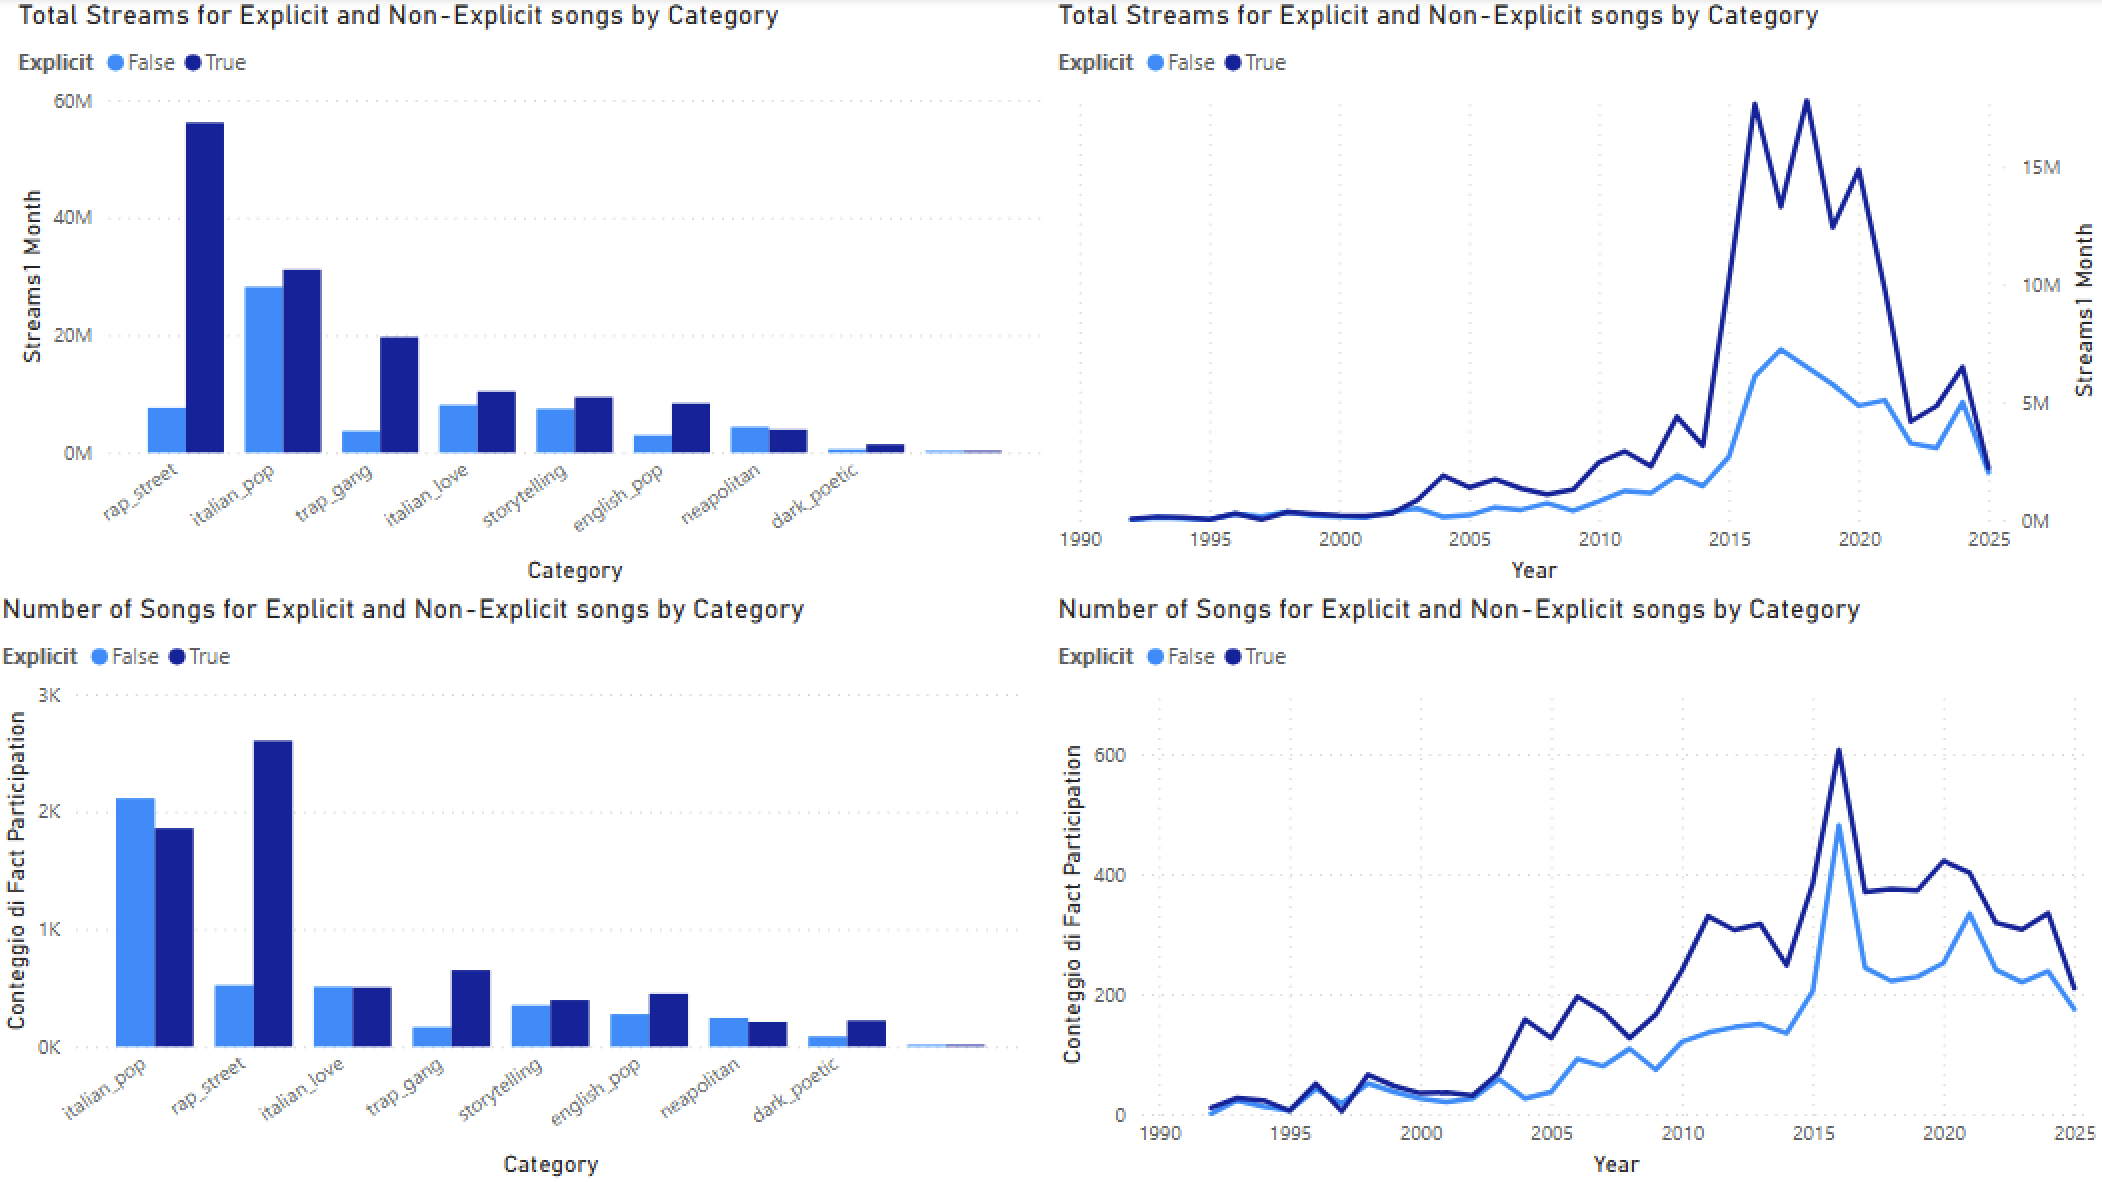
\includegraphics[width=1\textwidth]{Figures/Screenshot 2025-12-30 at 11.04.37.png}
    \caption{Grafici delle stream totali e numero canzoni explicit}
    \label{fig:ass_21}
\end{figure}

I due istogrammi sulla sinistra mostrano, rispettivamente, il numero
totale di stream per canzoni \emph{explicit} e \emph{non explicit}
per ciascuna categoria musicale.
Dall'analisi emerge come nella categoria \textit{rap\_street}
sia presente una marcata predominanza di tracce \emph{explicit},
che si riflette anche in un numero significativamente maggiore di stream.
Un comportamento analogo si osserva nella categoria \textit{trap\_gang},
mentre le restanti categorie presentano una distribuzione più
equilibrata tra contenuti \emph{explicit} e \emph{non explicit}.

I due grafici sulla destra rappresentano invece l'andamento temporale,
per anno, del numero totale di stream e del numero di canzoni,
distinguendo tra tracce \emph{explicit} e \emph{non explicit}.
Dal grafico relativo al numero di canzoni si osserva come la produzione
di contenuti \emph{explicit} e \emph{non explicit} risulti sostanzialmente
comparabile lungo l'intero periodo analizzato.
Tale equilibrio non si riflette però nel numero di stream, che mostra
una crescita molto pronunciata tra il 2015 e il 2020.
Questo incremento può essere interpretato come una conseguenza
dell'affermazione di generi particolarmente popolari in quel periodo,
tra cui \textit{trap\_gang} e un rinnovato interesse per il
\textit{rap\_street}.